\chapter{Task \#47: Spatial Covariance and Landau-Ginzburg Models for Embedded Empirical Networks}

\section{Introduction}

Statistical field theory offers a principled way to describe long-range correlations in spatially extended
systems through a small set of potential coefficients. Extending these ideas to
networks is difficult, but \emph{spatially embedded} networks provide a natural
starting point: their topology can be summarized by a \emph{graph kernel}: the probability $p(r)$ that two
nodes separated by a distance $r$ are connected, which plays the role of a two-point correlation function, and
can be compared with the covariance structure of a statistical field defined over the same space.

\noindent We consider a scalar Landau-Ginzburg (LG) theory with free energy
\begin{equation}
\mathcal{F}[\phi] = \int dx\left[\frac{\kappa}{2}(\nabla\phi)^2 + \frac{r_0}{2}\phi^2 + \frac{u}{4}\phi^4\right],
\end{equation}
with statistical weight $P[\phi]\propto e^{-\mathcal{F}[\phi]/T}$. In the Gaussian case ($u=0$) the connected
covariance is $G=TQ^{-1}$, where $Q=-\kappa\nabla^2+r_0$ is the precision operator and
$\xi=\sqrt{\kappa/r_0}$ the correlation length. We discretize the spatial domain on a regular grid of 
spacing $h$ and build $Q$ as the symmetric matrix
\begin{equation}
Q=\frac{\kappa}{h^2}L+r_0 I,
\end{equation}
where $L$ is the five-point graph Laplacian and $I$ the identity; the covariance is then obtained by sparse
matrix inversion, $G=TQ^{-1}$, and its radial profile is compared with the empirical kernel. The task is
therefore to test whether the empirical graph kernel can be reproduced by such a field theory, at three levels
of description: the empirical kernel fitted directly from the data, a \emph{homogeneous} LG model (global
coefficients), and a \emph{non-homogeneous} LG model whose mass varies in space,
$r(x)=r_0\bigl(1+\varepsilon\, m(x)\bigr)$, with $m(x)$ the local node-density anomaly.

\section{Data and Methods}

We use the GridKit dataset\footnote{B.~Wiegmans, \emph{GridKit: European and North-American extracts},
Zenodo, \texttt{10.5281/zenodo.47317} \cite{gridkit2016}.} of European and North-American high-voltage
power-grid extracts, with
stations as vertices and power lines as links. Node coordinates are projected to an equirectangular metric
system (centered on the network centroid, $R=6371$\,km). After collapsing multi-edges we restrict each network
to its largest connected component, obtaining $N=13\,478$ nodes and $E=16\,922$ links for Europe, and
$N=14\,990$ nodes and $E=18\,804$ links for North America ($\langle k\rangle\approx2.5$).

\noindent The homogeneous graph kernel is estimated by binning node pairs into logarithmically spaced radial
bins and taking $p(r)=\texttt{links}/\texttt{pairs}$ in each bin. We fit a family of parametric kernels (exponential,
Gaussian, power-law with cutoff, stretched exponential, and their product) by binomial log-likelihood over the
bins, selecting models by AIC. 
For the LG side we discretize the spatial domain, build the quadratic precision operator and obtain the covariance 
$G$ by sparse matrix inversion; its radial profile is averaged over source columns drawn from the grid interior 
and binned by distance with multiplicity weighting, and fitted to the empirical kernel by weighted least squares 
in log-log space. We fit the amplitude $A$ and the mass $r_0$; the stiffness and temperature are set to $\kappa=T=1$: 
they do not change the radial functional form, since they are absorbed by other parameters; 
so the single shape parameter is the correlation length $\xi=\sqrt{\kappa/r_0}=r_0^{-1/2}$. 
For the non-homogeneous level the mass varies over coarse spatial regions, $r(x)=r_0(1+\varepsilon m(x))$ with $m(x)$ the node-density
anomaly: we split the network into dense and sparse regions, fit the operator to each region's radial kernel
separately (obtaining $r_{\text{dense}}$, $r_{\text{sparse}}$), and invert the two relations
$r_g=r_0(1+\varepsilon m_g)$ for the coefficients $(r_0,\varepsilon)$. The quartic coupling is kept at $u=0$
(Gaussian baseline); a nonzero $u$ would merely renormalize the mass, an approximation we document in Sec.~\ref{sec:appendix2}, 
together with a more in-depth non-homogeneous analysis.

\section{Results}

Figure~\ref{fig:kernel_lg} shows the homogeneous graph kernel together with the parametric fits and the LG
reconstruction for the European network (North-American results reported in Fig.~\ref{fig:kernel_lg2}). 
The best parametric model for both networks is an exponential times power law,
$p(r)\propto e^{-r/\ell}(1+r/r_0)^{-\alpha}$, (fit results in Table~\ref{tab:res_fits}),
preferred over the exponential and the pure power-law cutoff by AIC
(Table~\ref{tab:kernel_models}).

\begin{figure}[htbp]
    \centering
    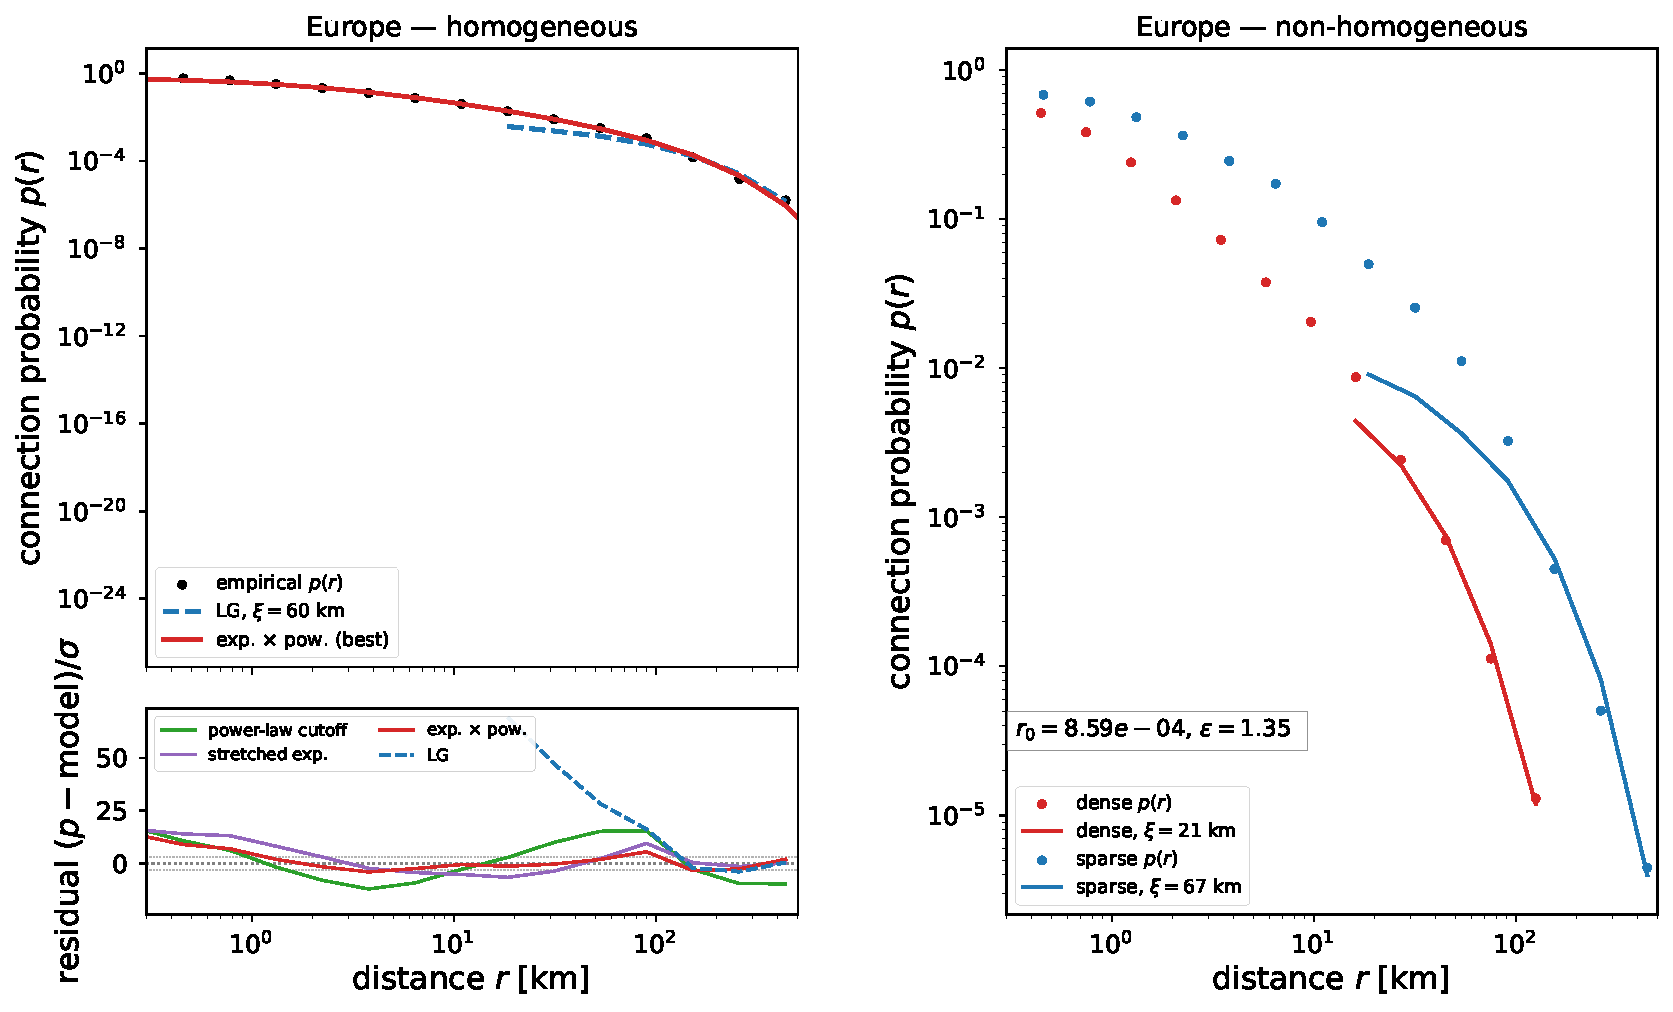
\includegraphics[width=0.98\textwidth]{./figures/task_47/task_47_kernel_lg_europe.pdf}
    \caption{Fit results for the European network. Left: empirical homogeneous kernel $p(r)$ with the best
    parametric fit and the homogeneous Landau-Ginzburg operator $Q=(\kappa/h^2)L+r_0I$ (dashed); below it, the
    standardized residual $(p-\mathrm{model})/\sigma$ (per-bin binomial standard error $\sigma$) for the
    power-law-capable kernels (power-law cutoff, stretched exponential, exponential-times-power-law) and the
    operator, with a zero line and a $\pm3\sigma$ band; the pure exponential-decay kernels (exponential,
    Gaussian) are off-scale in the tail and omitted. Right: the non-homogeneous
    decomposition into dense (red) and sparse (blue) regions, each with its own operator fit; the inferred
    non-homogeneous coefficients $(r_0,\varepsilon)$ are reported. North American results shown in
    Fig.~\ref{fig:kernel_lg2}.}
    \label{fig:kernel_lg}
\end{figure}

\noindent The homogeneous LG model reproduces the kernel well at high and intermediate distances ($r\ge\xi$), 
but it is not representative at lower distances (see Figs.~\ref{fig:kernel_lg} and \ref{fig:kernel_lg2}). 
This model is limited by the grid spacing $h=15$km, and it can predict only above this distance;
furthermore, the fitting of the model is based on Least Squares, weighted 
on pair counts. Since the number of pairs $\propto r^2$, the tail dominates the fit, and the smaller data are less represented.
The discrete covariance of the massive Gaussian operator decays as $e^{-r/\xi}/\sqrt{r}$, falling faster than the
empirical power-law tail. The shape mismatch would be present also changing the grid spacing to smaller values 
(at the price of a massive increase in computational cost of the fit), and this is the signature that a Gaussian 
field theory with a single mass cannot capture the heavy-tailed spatial organization of the power grid.

\noindent The non-homogeneous level quantifies the spatial heterogeneity directly: dense regions are characterized by a
much shorter correlation length than sparse ones, $\xi_{\text{dense}}\approx21$\,km versus
$\xi_{\text{sparse}}\approx67$\,km for Europe. Inverting the mass relation gives $r_0\approx8.6\times10^{-4}$
and $\varepsilon\approx1.35$ (Europe); a strongly density-dependent mass with $\varepsilon>0$: urbanized
regions (positive density anomaly) carry a larger mass and hence connect over shorter scales, while rural
regions sustain long transmission lines. The North-American decomposition shows the same qualitative pattern and
is reported in the Supplementary Material. The density maps (Fig.~\ref{fig:density}) confirm that the dense/sparse
split corresponds to a genuine geographic, not merely statistical, partition.

\section{Discussion}

The three levels of description form a coherent hierarchy. The empirical graph kernel establishes a heavy-tailed,
power-law baseline (an exponential times power-law decay is preferred by AIC). The homogeneous LG model captures
the correct correlation length but, being a massive
Gaussian theory, is constrained to exponential decay and therefore underestimates the tail. The non-homogeneous
model, with a density-dependent mass, recovers the local correlation structure and identifies dense and
sparse regions as carrying distinct effective masses. In this sense the field-theoretic description does capture
nontrivial spatial organization beyond a simple distance-decay kernel: the dependence of the correlation length
on local density is precisely the kind of information a single homogeneous kernel discards.

\noindent Several approximations limit the analysis and are documented explicitly. (i) The equirectangular projection is
adequate at continental scale but not conformal; a proper projected CRS would refine the distance estimates.
(ii) The discrete operator has no covariance for distances below the lattice spacing $h$: the ultraviolet
divergence of the continuum Green's function is regularized by $h$, so the model is only matched for $r$ above a
cutoff $r_{\min}=h$. The empirical kernel is nevertheless measured below $h$ (down to $\sim0.1$\,km), so the
smallest bins are shown but not described by the field theory. (iii) The
quartic term is set to $u=0$; treating $u>0$ (mean-field or perturbatively) would renormalize $r_0$ but not alter
the qualitative exponential decay. (iv) Power grids are quasi-one-dimensional (they follow geographic
corridors), so the isotropic two-dimensional covariance is an idealized reference rather than an exact model.
Finally, the non-homogeneous inference is performed with a two-region density split; a continuous $m(x)$ over a
finer spatial grid is a natural extension.

\newpage

\section{Supplementary Material}

\label{sec:appendix2}

\subsection{Fit Results}
\begin{table}[htbp]
    \centering
    \begin{tabular}{l|ccc}
        \toprule
        \textbf{Network} & \textbf{$\ell$} [km] & \textbf{$r_0$} [km] & \textbf{$\alpha$} \\
        \midrule
        Europe       & $75$ & $1.9$ & $1.4$\\
        North America          & $81$ & $2.7$ & $1.6$\\
        \bottomrule
    \end{tabular}
    \caption{Fit parameters for the exponential times power law model (best model) for both networks.}
    \label{tab:res_fits}
\end{table}

\begin{figure}[htbp]
    \centering
    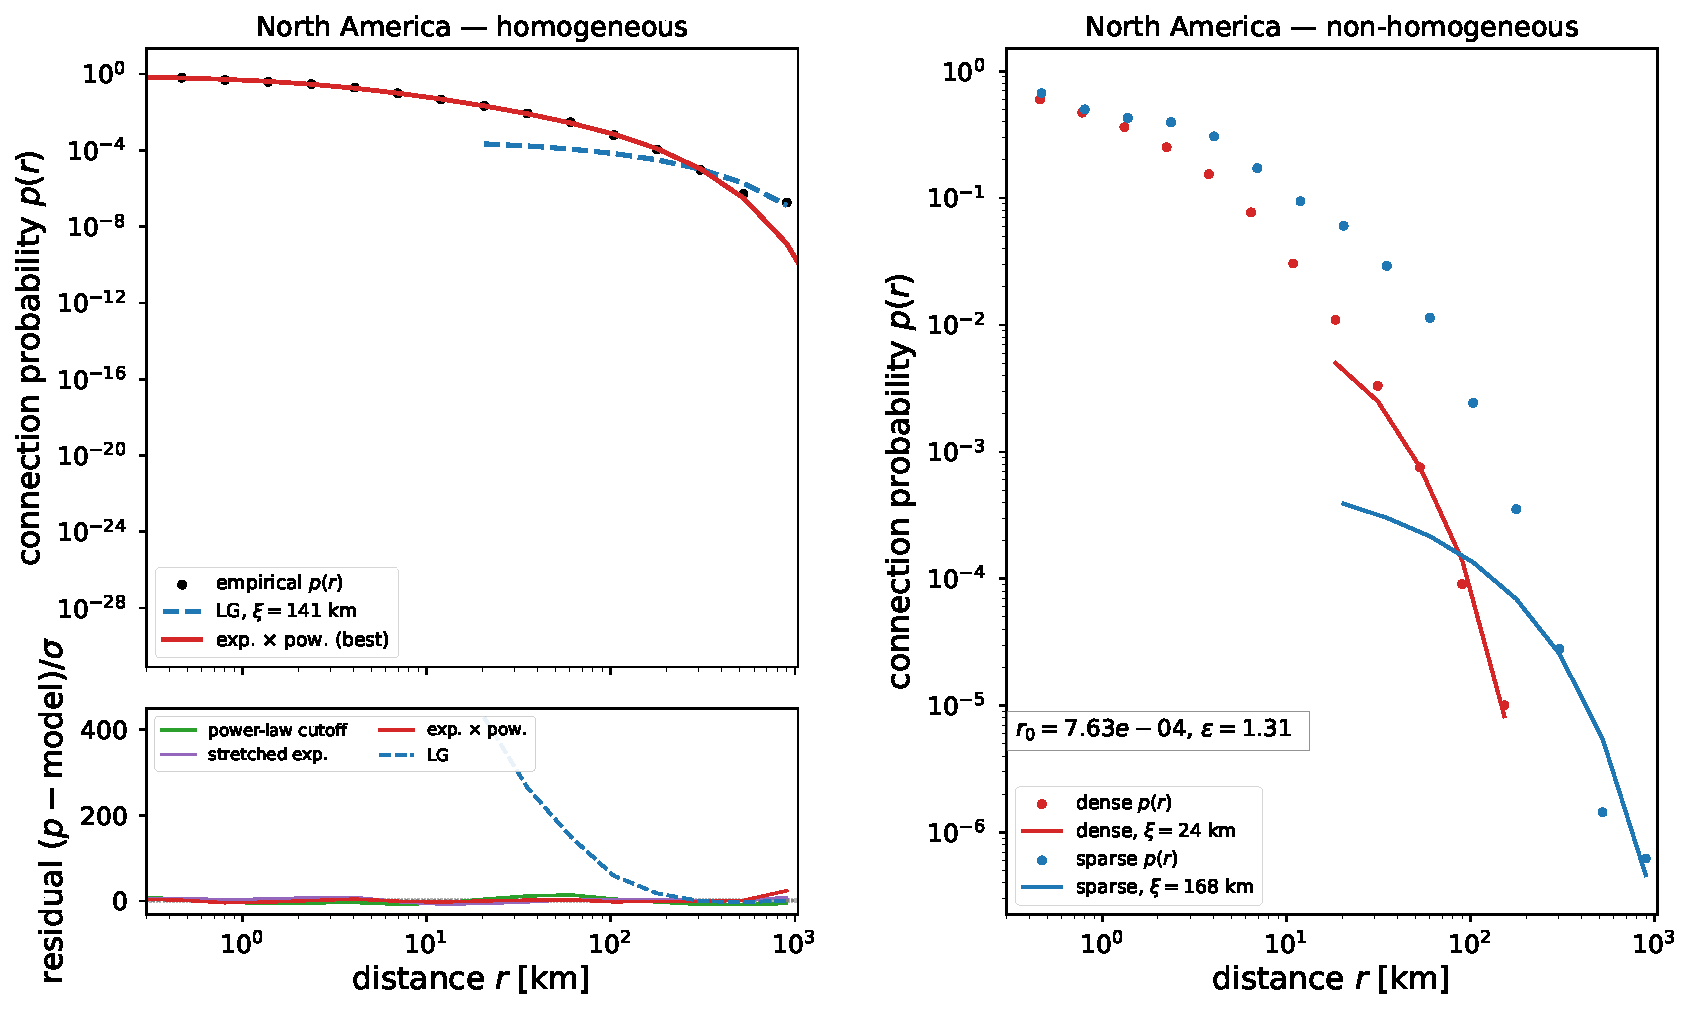
\includegraphics[width=0.98\textwidth]{./figures/task_47/task_47_kernel_lg_north_america.pdf}
    \caption{Fit results for the North American network. Left: empirical homogeneous kernel $p(r)$ with the best
    parametric fit and the homogeneous Landau-Ginzburg operator $Q=(\kappa/h^2)L+r_0I$ (dashed); below it, the
    standardized residual $(p-\mathrm{model})/\sigma$ (per-bin binomial standard error $\sigma$) for the
    power-law-capable kernels (power-law cutoff, stretched exponential, exponential-times-power-law) and the
    operator, with a zero line and a $\pm3\sigma$ band; the pure exponential-decay kernels (exponential,
    Gaussian) are off-scale in the tail and omitted. Right: the non-homogeneous
    decomposition into dense (red) and sparse (blue) regions, each with its own operator fit; the inferred
    non-homogeneous coefficients $(r_0,\varepsilon)$ are reported.}
    \label{fig:kernel_lg2}
\end{figure}

\noindent The homogeneous LG operator gives $\xi\approx141$\,km with
$R^2=0.59$, a weaker fit than Europe because the network spans larger distances and its power-law tail is more
prominent (Table~\ref{tab:lg_params}). The non-homogeneous split yields $\xi_{\text{dense}}\approx24$\,km versus
$\xi_{\text{sparse}}\approx168$\,km, inverting to $\varepsilon\approx1.31$.

\begin{table}[htbp]
    \centering
    \begin{tabular}{l|c|cc|cc}
        \toprule
        \textbf{Model} & \textbf{DOF} & \textbf{NLL (EU)} & \textbf{AIC    \tablefootnote{Given a statistical model with $k$ estimated parameters, the Akaike Information Criterion is defined as $\text{AIC}=2k-2\text{ln}(L)$, where $L$ is the maximized value of the Likelihood function for the model.} (EU)} & \textbf{NLL (NA)} & \textbf{AIC (NA)} \\
        \midrule
        exponential       & $2$ & $6.681\times10^{4}$ & $1.336\times10^{5}$ & $6.959\times10^{4}$ & $1.392\times10^{5}$ \\
        gaussian          & $2$ & $7.649\times10^{4}$ & $1.530\times10^{5}$ & $8.029\times10^{4}$ & $1.606\times10^{5}$ \\
        power-law cutoff  & $3$ & $6.033\times10^{4}$ & $1.207\times10^{5}$ & $6.300\times10^{4}$ & $1.260\times10^{5}$ \\
        stretched exp.    & $3$ & $6.006\times10^{4}$ & $1.201\times10^{5}$ & $6.274\times10^{4}$ & $1.255\times10^{5}$ \\
        exp. $\times$ pow.& $4$ & $5.974\times10^{4}$ & $1.195\times10^{5}$ & $6.258\times10^{4}$ & $1.252\times10^{5}$ \\
        \bottomrule
    \end{tabular}
    \caption{Model selection for the homogeneous graph kernel (binomial log-likelihood). The
    exponential-times-power-law model is preferred for both networks. Negative Log Likelihood (NLL) and AIC
    are reported as fit quality estimates.}
    \label{tab:kernel_models}
\end{table}

\begin{table}[h!]
    \centering
        \begin{tabular}{l|cc|cccc}
        \toprule
        \textbf{Network}& $\xi$ (km) & $r_0^{\text{hom}}$ (km$^{-2}$) & $r_0^{\text{non-hom}}$ (km$^{-2}$) & $\xi_{\text{d}}$ (km) & $\xi_{\text{s  }}$ (km) & $\varepsilon$ \\
        \midrule
        Europe        & $60.1$ & $2.77\times10^{-4}$ & $8.59\times10^{-4}$ & $21.4$ & $66.5$ & $1.35$ \\
        North America & $140.7$ & $5.05\times10^{-5}$ & $7.63\times10^{-4}$ & $24.0$ & $167.9$ & $1.31$ \\
        \bottomrule
    \end{tabular}
    \caption{Inferred Landau-Ginzburg parameters. Homogeneous: correlation length $\xi$ and mass
    $r_0^{\text{hom}}=\kappa/\xi^2$ ($\kappa=1$), fitted from the discretized operator $Q=(\kappa/h^2)L+r_0 I$.
    Non-homogeneous: density-conditioned correlation lengths and the
    baseline mass of $r(x)=r_0^{\text{non-hom}}(1+\varepsilon m(x))$, together with the coupling
    $\varepsilon$.}
    \label{tab:lg_params}
\end{table}

\subsection{Node Density of the networks}

\begin{figure}[h!]
    \centering
    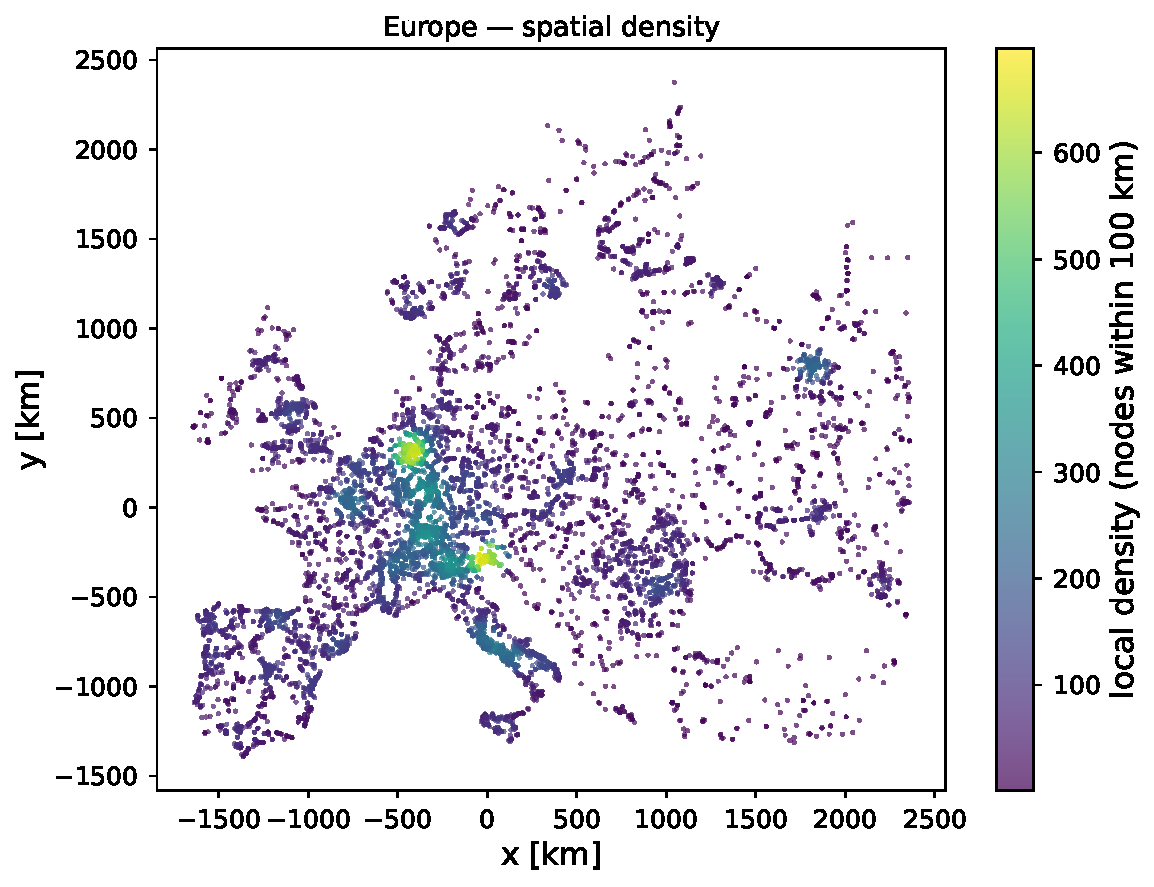
\includegraphics[width=0.49\textwidth]{./figures/task_47/task_47_density_map_europe.pdf}\hfill
    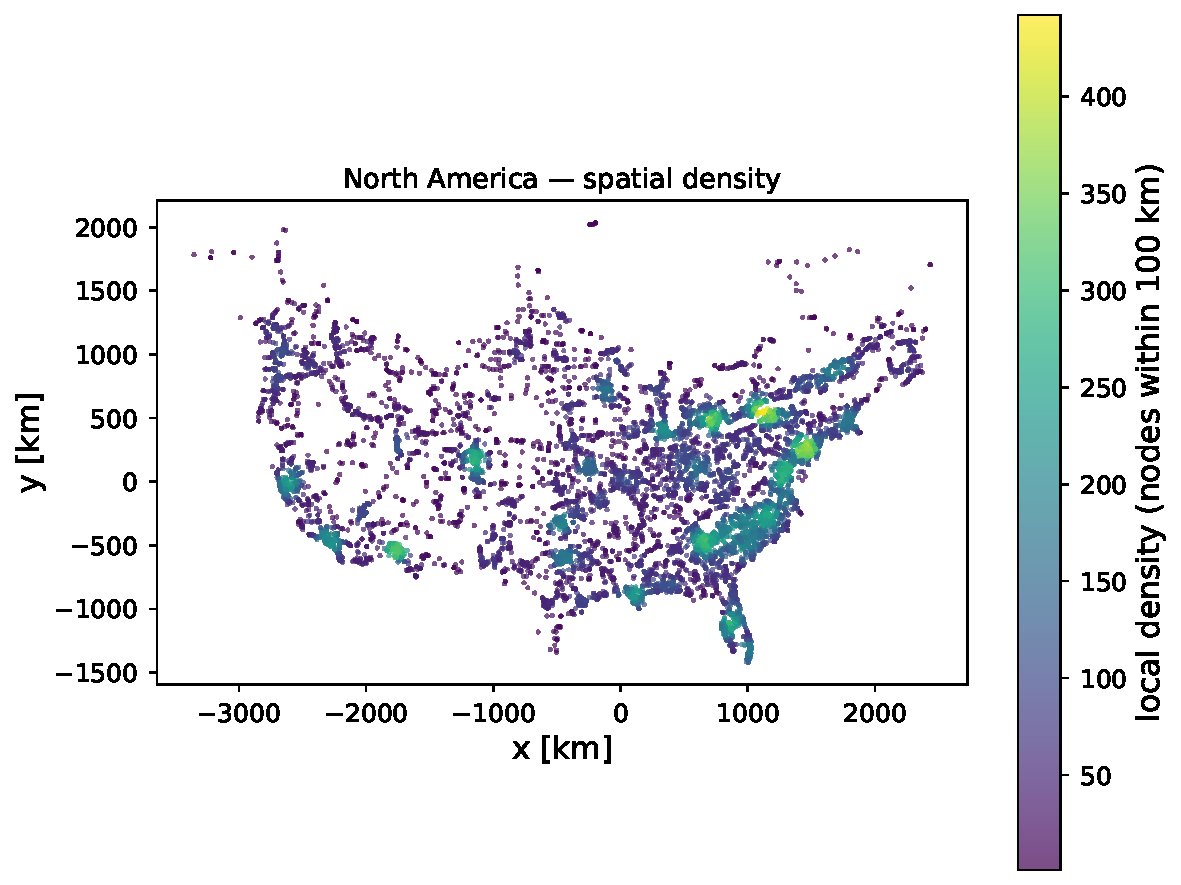
\includegraphics[width=0.49\textwidth]{./figures/task_47/task_47_density_map_north_america.pdf}
    \caption{Local node density (neighbours within $100$\,km) for Europe (left) and North America (right). The
    dense/sparse partition used for the non-homogeneous LG model is a genuine spatial structure.}
    \label{fig:density}
\end{figure}

\subsection{Perturbative extension: non-homogeneous mass and quartic coupling}

\noindent This section tries to make perturbative level precise. \emph{What is computed}: (i) the first-order (in
$\varepsilon$) correction $\delta G$ to the covariance induced by a spatially varying mass, and (ii) the
one-loop (in $u$) mass renormalization of the quartic vertex. \emph{What analysis is performed}: the
$\varepsilon$-expansion is validated against the exact inversion (truncation error $\propto\varepsilon^2$), the
radial average of $\delta G$ is shown to be suppressed (so $\varepsilon$ is identified from the
density-conditioned kernels rather than the radial profile), and the vacuum variance $\langle\phi^2\rangle_0$ is
evaluated to bound the admissible $u$. \emph{What results are reached}: a positive coupling
$\varepsilon\approx0.83$ (Europe) and $0.44$ (North America), consistent in sign with the two-region inversion
($\varepsilon\approx1.3$); a UV-sensitive $\langle\phi^2\rangle_0\approx111$/$142$; and a quartic coupling
$u\sim8\times10^{-7}$ that already shifts the mass by $r_0$, showing the $\phi^4$ vertex is strongly relevant in
$d=2$ while leaving the exponential tail qualitatively unchanged.

\noindent The non-homogeneous mass $r(x)=r_0\bigl(1+\varepsilon m(x)\bigr)$ and the quartic coupling $u$ are treated
perturbatively around the homogeneous Gaussian operator, so that the precision matrix is factorized \emph{once}
and every parameter value is explored without a further decomposition. The local density anomaly is discretized
on the same regular grid: the number of \emph{network vertices} within $100$\,km of each grid site (a KD-tree
range query, the same estimator used for the node-level density, standardized over grid sites), giving a
continuous field $m(x)$. The precision matrix splits as
\begin{equation}
Q(\varepsilon)=Q_0+\varepsilon M,\qquad M=r_0\,\mathrm{diag}\,m(x),\qquad
Q_0=\frac{\kappa}{h^2}L+r_0 I,
\end{equation}
and the covariance expands as $G=TQ^{-1}=G_0+\delta G+\mathcal{O}(\varepsilon^2)$, where
\begin{equation}
\delta G=-\varepsilon\,T\,Q_0^{-1}M\,Q_0^{-1},
\qquad\text{or, per source column,}\quad
\delta G\,e_s=-\varepsilon\,Q_0^{-1}\bigl(r_0\,m(x)\odot g_0\bigr),
\end{equation}
with $g_0=TQ_0^{-1}e_s$ (the sampling temperature $T$ cancels). A single sparse LU factorization of $Q_0$
therefore supplies the $\mathcal{O}(\varepsilon)$ correction at the cost of one extra back-substitution per
source column. The radial average of $\delta G$ is strongly suppressed: the anomaly has zero mean, so only the
spatial variation of the smoothing kernel contributes (the radial correction reaches $\approx12\%$ of the peak
for Europe at the fitted $\varepsilon$; Fig.~\ref{fig:kernel_lg}); this is precisely why $\varepsilon$ is
identified from a \emph{density-conditioned} observable (the dense- and sparse-restricted kernels) rather than
from the radial kernel alone. The truncation is second order: at $\varepsilon=0.05$ the perturbative profile
differs from the exact inversion by $\lesssim2\times10^{-5}$ relative to the peak, growing $\propto\varepsilon^2$.

\noindent Fitting $(A,\varepsilon)$ (with $r_0$ fixed at its homogeneous value) to the dense- and
sparse-conditioned kernels gives $\varepsilon\approx0.83$ (Europe) and $\varepsilon\approx0.44$ (North
America), consistent in sign with the two-region inversion ($\varepsilon\approx1.3$): a positive density anomaly
carries a larger effective mass. The smaller magnitude reflects two documented approximations: the fit uses a
single global amplitude $A$, whereas dense and sparse populations have markedly different overall connection
rates, and the standardized grid field $m(x)$ additionally samples empty space that the node-level anomaly does
not.

\noindent To first order in $u$ the only effect of the $\phi^4$ term is a renormalization of the mass,
\begin{equation}
r_{\mathrm{eff}}=r_0+3u\,\langle\phi^2\rangle_0,\qquad
\langle\phi^2\rangle_0=T\,\frac{1}{N}\operatorname{tr}Q_0^{-1},
\end{equation}
the factor $3$ counting the tadpole contractions of the $u/4\,\phi^4$ vertex. The vacuum variance
$\langle\phi^2\rangle_0$ is ultraviolet-sensitive: on the lattice it evaluates to $\approx111$ (Europe) and
$\approx142$ (North America). The quartic coupling is therefore
strongly relevant in $d=2$: a shift as large as $\delta r=r_0$ already requires
$u\sim r_0/\bigl(3\langle\phi^2\rangle_0\bigr)\approx8\times10^{-7}$. This makes quantitative the statement of
the main text that $u>0$ only renormalizes the mass (shrinking $\xi=\sqrt{\kappa/r_{\mathrm{eff}}}$) without
altering the qualitative exponential decay.

\newpage
